\chapter{Motivation} \label{chapter:MOTIVATION}

In the Lively Kernel, programmers can create applications by manipulating and composing graphical parts.
This chapter demonstrates the development of such parts and related recovery needs by example.


\section{Part Development By Example}

To exemplify how developers work directly on objects in Lively, we will outline the process of adding a new feature to the Lively Kernel's Object Editor.

\begin{figure}[h]
    \centering
    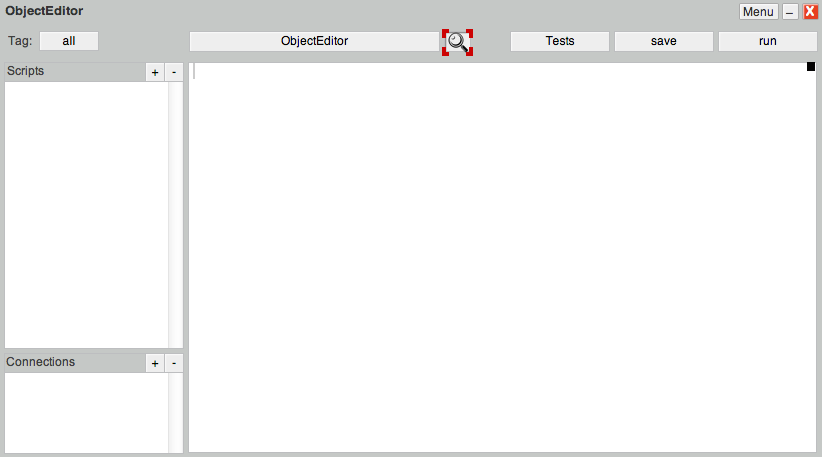
\includegraphics[width=\textwidth]{figures/3_motivation/1_magnifierButton.png}
    \caption{The Object Editor with its magnifier button highlighted with a red outline.}
    \label{fig:MagnifierButton}
\end{figure}

The editor itself has been been developed by composing and editing graphical objects directly.
For this reason, we do not have to adapt any source code modules to change the editor, but rather manipulate particular objects directly.
The new feature we add in this example is a magnifier button that can show the editor's current editing target.
Adding this feature requires to create and add a new button morph to the editor, as shown in Figure~\ref{fig:MagnifierButton}.

The magnifier button implements two features: First, when a programmer hovers over the button, the Object Editor's current target object is highlighted through a transparent overlay. Second, when a programmer clicks the button, the current target selection is revoked and the programmer can visually select the new target of the editor.
This example covers the first of these two behaviors, which is also shown in Figure~\ref{fig:MagnifierBehavior} for an Object Editor currently targeting the character of a game.

\begin{figure}[h]
    \centering
    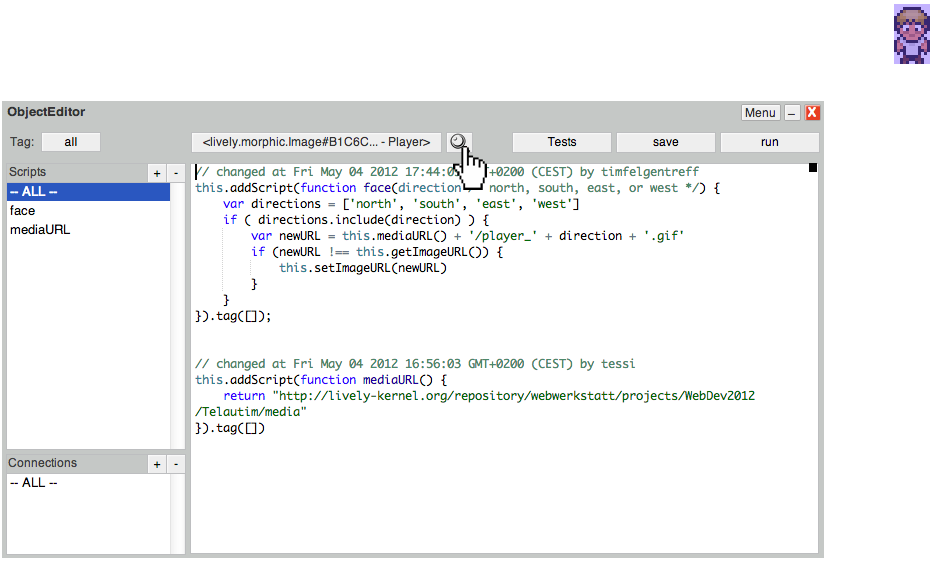
\includegraphics[width=0.8\textwidth]{figures/3_motivation/2_magnifierBehavior.png}
    \caption{Hovering the Object Editor's magnifier button highlights the current target object.}
    \label{fig:MagnifierBehavior}
\end{figure}

\paragraph{Manipulating the Button Morph}
Before we implement the button's behavior, we first create the button's visual appearance, as shown in Figure~\ref{fig:ButtonBuilding}.
A basic button, as visible in \textcircled{1}, can be found in the Parts Bin repository.
We can use the button's halos and, in particular, the resize tool in \textcircled{2} to give the button a smaller and square extent.
Next, we can load an image showing a magnifier.
Using drag and drop we can add the image to the button, as done in \textcircled{3}.
Dropping a morph onto another structurely connects morphs in Lively.
That is, moving the button around will also move the image accordingly, while saving will also persist both.
Subsequentely, we can add the result of these direct manipulations, visible in \textcircled{4}, to the object editor.

\begin{figure}[h]
    \centering
    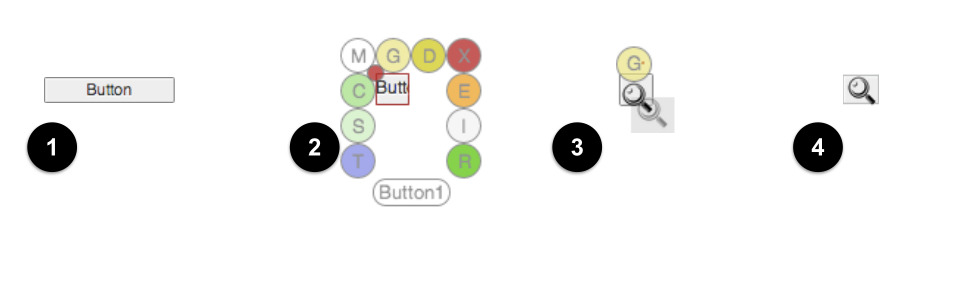
\includegraphics[width=\textwidth]{figures/3_motivation/3_buildingTheButton.png}
    \caption{Directly manipulating a button morph.}
    \label{fig:ButtonBuilding}
\end{figure}

All these changes are made directly to the state of objects: the button morph, the magnifier image morph, and the editor morph.
When programmers edit parts directly in this way, they often see the effects of their actions immediately.
For example, when adding the button morph to the Object Editor, where the button will be is visible at all times.
Developers do not need to run any code to check the resulting appearance.

\paragraph{Scripting the Button Morph}
Next, the magnifier button needs its behavior.
We add scripts to the button that lay a translucent rectangle over the current target.
The implementation of this could include the following: The button knows a transparent rectangle. When the mouse enters the button, the button rezises and adds the rectangle to the world at the position of the target. When the mouse leaves the button, the button removes the rectangle from the world.
This behavior is, thus, triggered from two scripts of the button morph, which are the the scripts \lstinline{onMouseMove} and \lstinline{onMouseOut}.

When developing such scripts with an Object Editor, the editor allows to evaluate code in the context of its target.
So, when developers want to test a script or even just specific lines of code, they can often try the behavior directly with the actual target.


\section{Recovery Needs When Developing Parts}

While manipulating objects directly, developers might make changes that they subsequentely want to undo.

In the previous example developers could, for example, make any of the following mistakes:

\begin{itemize}
    \item accidentally grap and move a morph such as the new button and, thereby, change the carefully arranged layout.
    \item close a morph such as the Object Editor, which contains the new button, and, thus, lose meaningful unsaved changes.
    \item introduce an an error or a decrease in performance with an edit to a script.
\end{itemize}

Besides these accidental mistakes, well-intentioned changes can also turn out to be inappropriate.
When fine-tuning the visual appearance of a morph, for example, a developer might make many changes to the sizes, the positions, and the colors of morphs, only to decide later that a particular intermediate version was most appealing.
Developers can also change objects through a code snippet from a temporary workspace.
Such a snippet can change any number of properties of many objects at once, so re-establishing a previous state would be a laborious task.

Potentially undesirable changes might also be introduced when programmers explore the behavior of objects by evaluating their scripts.
For example, the Object Editor always manipulates the scripts of a specific object and developers can evaluate code directly for that target object.
While such evaluation might help to understand the effects of particular code, it might also change the state of objects permanently.

A programmer could edit the button's \lstinline{onMouseMove} script and afterwards could evaluate a few lines of code to quickly test his changes.
These lines, as shown in Figure~\ref{fig:onMouseOverScript}, would, however, add the rectangle to the current target, without regard to the conditions usually checked before and without setting the state as done right after the selection in the script.
Thus, while evaluating this selection allows to test the highlighting behavior, it leaves the system in a state that it would normally be in.

\begin{figure}[h]
    \centering
    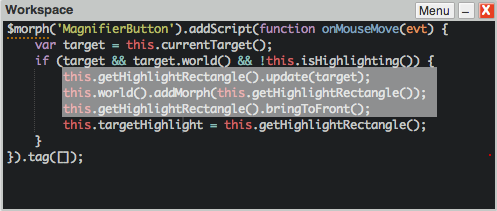
\includegraphics[width=0.7\textwidth]{figures/3_motivation/4_workspaceDoIt.png}
    \caption{The button's \lstinline{onMouseMove} script with a text selection.}
    \label{fig:onMouseOverScript}
\end{figure}

The given examples show that there are many situations in which developers might want to undo some of their operations.
In programming systems like the Lively Kernel, where programmers often work at runtime on objects, the development state consists of the state of objects.
Even classes and modules are objects in the Lively Kernel.
That is, changes are always made to objects.
More precisely, changes are always made to the \emph{state of objects} as even functions are also just properties of objects.

\begin{figure}[h]
    \centering
    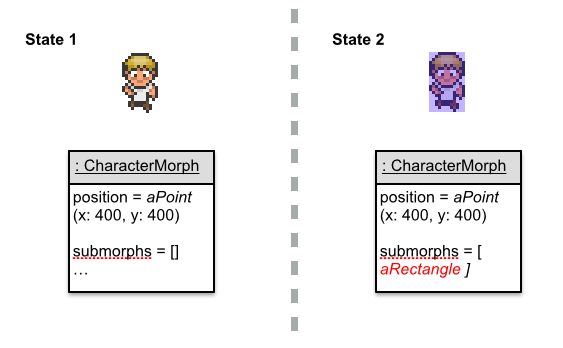
\includegraphics[width=0.7\textwidth]{figures/3_motivation/5_stateChanges.png}
    \caption{Adding a submorph changes the state of a morph.}
    \label{fig:changedCharacter}
\end{figure}

If, for example, the text selection in Figure~\ref{fig:onMouseOverScript} gets evaluated, the world object is changed.
In particular, its collection of submorphs is altered.
The world has now one more submorph, as shown in Figure~\ref{fig:changedCharacter}.

To undo the change and re-establish the previous version of the character, the world object needs to have its previous state.
The \lstinline{submorphs} property needs to be as it previously was.
Similarly, when the state of all objects is preserved and can be re-established on demand, previous development states can be recovered whenever recovery is necessary.
